\subsection{Démonstration numérique}

\paragraph{} Dans cette section, nous nous restreignons au cas d'un potentiel en double puits avec un forçage uniforme, $h(x)=1$.
Nous faisons la simulation numérique de la dynamique stochastique \ref{SDE_particule} et confronterons les résultats aux expressions analytiques de la section précédente. La simulation numérique a l'avantage de nous permettre de sortir des limites de validité des approximations faites dans la partie analytique et d'étendre ainsi l'exploration du phénomène.


\subsubsection{Cas d'un double puits de potentiel}

Le potentiel considéré -- voir figure \ref{fig:potentiel_double_puits} -- est donné par

\begin{equation}\label{potentiel_double_puits}
U(x) = -\frac{\lambda}{2}x^2 + \frac{1}{4} x^4, \qquad \lambda>0.
\end{equation}
les minimas sont $x_\pm = \pm \lambda^{1/2}$ et sont séparés par une barrière de potentiel en $x=0$ d'une hauteur $\Delta U_\pm = \lambda^2/4$. Les taux de transitions en l'absence de forçage valent

\begin{equation}\label{r_dbpuits}
	r = r_\pm = \frac{\lambda}{\sqrt 2\pi} \exp\left( -\frac{\lambda^2}{2 q^2} \right) 
\end{equation}
et l'amplitude de la réponse $p_+(t) = p_+ + A\cos(\omega t+\varphi)$ à un petit forçage est

\begin{equation}\label{pi_dbpuits}
	|A| = |\epsilon \pi_+| = \frac{\epsilon}{q^2} \frac{\lambda^{1/2}}{\sqrt{1+\omega^2/(2r)^2}}.
\end{equation}

%Le décalage de phase vaut quant à lui $\Delta\phi = \arctan(-\omega/(2r))$.

\begin{figure}
	\centering
	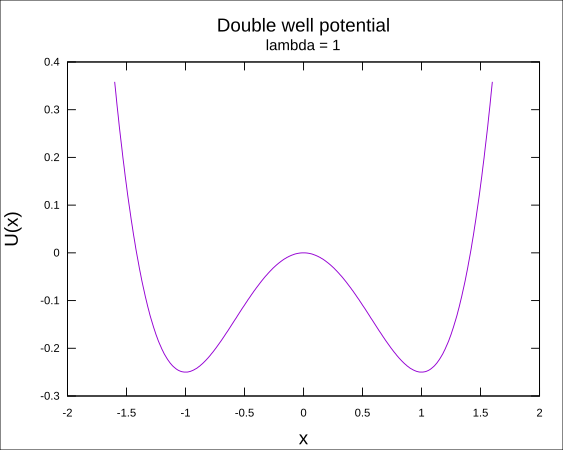
\includegraphics[width=0.8\linewidth]{figures/potential}
	\caption{Potentiel en double puits utilisé pour l'application numérique.}
	\label{fig:potentiel_double_puits}
\end{figure}


\subsubsection{Simulation du processus stochastique}

\paragraph{} La dynamique stochastique \ref{SDE_particule} s'intègre en discrétisant le temps en pas $dt$. L'équation discrétisée devient

\begin{equation}\label{SDE_discrete}
	x_{n+1} = \frac{\partial U(x_n)}{\partial x} dt + \epsilon h(x_n) \cos(\omega t + \phi) dt + \sqrt{q^2 dt} \,G_n,
\end{equation}
où la variable $G_n$ est une variable aléatoire suivant une distribution normale avec 

\begin{equation}\label{G_n}
\begin{split}
	&\langle G_n \rangle = 0,\\
	&\langle G_nG_{n'} \rangle = \delta_{nn'}.
\end{split}
\end{equation}

\paragraph{} Dans les limites de validité du développement de la section précédente, ici $\epsilon \ll q^2 \lambda^{-1/2}$, la simulation du processus pour le potentiel en double puits montre des transitions aléatoires entre les puits -- voir figure \ref{fig:trajectory_random}. Ceci est dû au fait que la réponse est trop petite pour être vue sur le graphique de la trajectoire. Dans la section suivante, nous allons intégrer sur des temps plus long et prendre la transformée de Fourier du signal afin d'extraire la réponse au premier ordre. Contrairement au développement perturbatif de la théorie, la simulation nous permet d'analyser la réponse non-linéaire du système pour de plus grands forçages. La figure \ref{fig:trajectory_resonant} montre un exemple de synchronisation de la trajectoire avec le forçage. Bien que le forçage soit assez grand pour causer des effets non-linéaires, la synchronisation est bien causée par le bruit dans le système. La trajectoire déterministe pour un même forçage ne donne pas de telle transitions, la réponse déterministe étant bien trop petite -- voir figure \ref{fig:trajectory_deterministic_small}.


\begin{figure}[p]
	\centering
	
	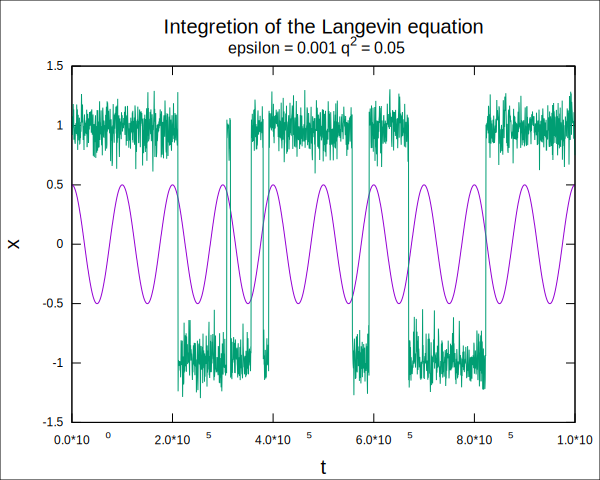
\includegraphics[width=0.8\linewidth]{figures/trajectory_random}
	\caption{Trajectoire pour un petit forçage. La réponse $\pi_+$ est linéaire et beaucoup plus petite que la probabilité à l'ordre zéro. Les transitions sont donc encore aléatoires. L'amplitude du forçage (en mauve) est ajustée pour des raisons de visibilité.}
	\label{fig:trajectory_random}
	
	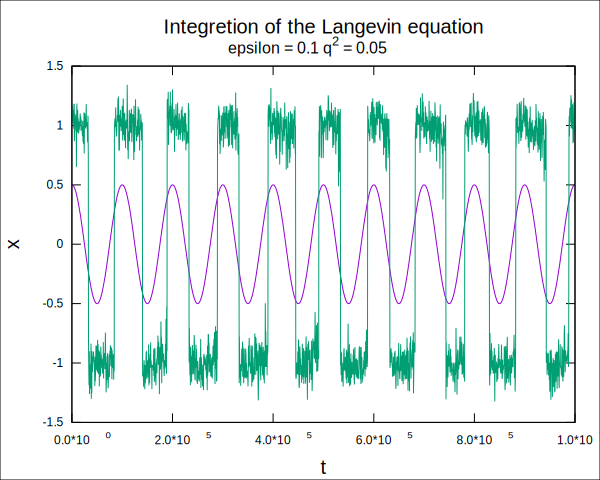
\includegraphics[width=0.8\linewidth]{figures/trajectory_resonant}
	\caption{Trajectoire pour un forçage d'amplitude comparable à $q^2$. La réponse $\pi_+$ est non-linéaire et efface le comportement à l'ordre zéro. Les transitions sont synchronisées avec le forçage. Le décalage de phase est très net sur cette image. L'amplitude du forçage (en mauve) est ajustée pour des raisons de visibilité.}
	\label{fig:trajectory_resonant}
\end{figure}

\begin{figure}[p]
	\centering
	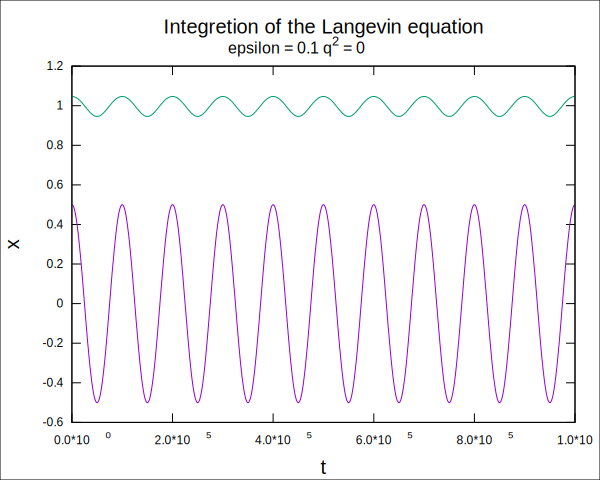
\includegraphics[width=0.8\linewidth]{figures/trajectory_deterministic_small}
	\caption{Réponse déterministe au forçage externe. Cette image montre que la synchronisation observée pour $\epsilon = 0.1$ -- voir figure \ref{fig:trajectory_resonant} -- est bien due au mécanisme de résonance stochastique. L'amplitude du forçage (en mauve) est ajustée pour des raisons de visibilité.}
	\label{fig:trajectory_deterministic_small}

	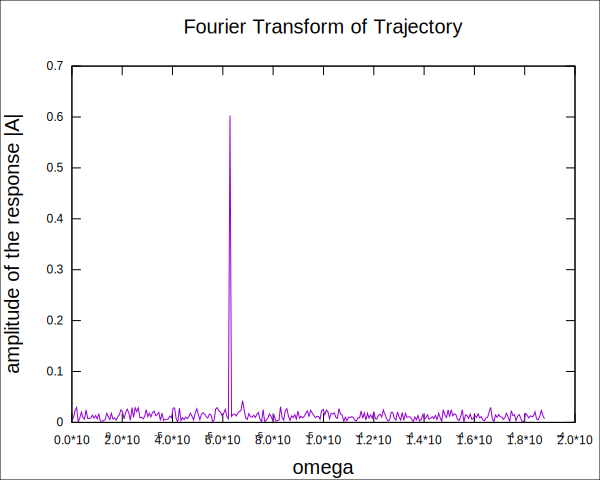
\includegraphics[width=0.8\linewidth]{figures/spectrum_resonant}
	\caption{Transformée de Fourier de la trajectoire résonante de la figure \ref{fig:trajectory_resonant}.}
	\label{fig:spectrum_resonant}
\end{figure}

\subsubsection{Analyse de Fourier et amplification en fonction du bruit}

\begin{figure}
	\centering
	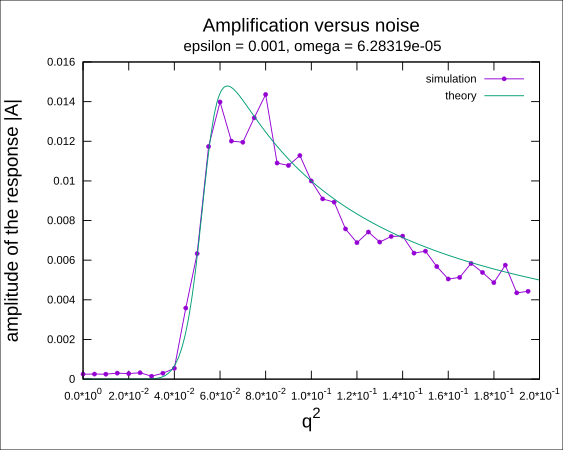
\includegraphics[width=0.8\linewidth]{figures/amplification_versus_noise}
	\caption{Amplitude de la réponse linéaire à un petit forçage en fonction de l'intensité du bruit. Nous pouvons clairement observer le phénomène de résonance stochastique dû à la présence de bruit dans le système.}
	\label{fig:amplification_versus_noise}
\end{figure}

\paragraph{} Pour pouvoir comparer les prévisions analytiques avec la simulation numérique, il faut pouvoir extraire l'amplitude de la réponse au premier ordre. Nous réalisons cela en intégrant le système sur un temps assez long pour avoir une résolution assez bonne sur la probabilité de résidence en chaque puits à l'ordre $\epsilon$ et prenons ensuite la transformée de Fourier de la trajectoire. Nous sommes intéressés par le coefficient de Fourier associé à la fréquence du signal.

\paragraph{} Numériquement, nous faisons une transformée de Fourier discrète des positions $\{f_j\}_{j=0}^N$ enregistrés à intervalle régulier depuis la trajectoire $f(t)$. L'expression des valeurs discrétisées de la  transformée de Fourier est 

\begin{equation}\label{f_hat_k}
	\hat f_k = \frac{1}{\sqrt{2\pi}} \sum_{j=0}^{N} \Delta t f_j e^{-i\omega t}.
\end{equation}
Les temps et fréquences sont discrétisés de sorte à ce que $t=j\Delta t$ et $\omega = k\Delta \omega$. L'intervalle des fréquences est relié à l'intervalle temporel par $\Delta \omega = 2\pi/(N\Delta t)$. De cette manière, nous pouvons réaliser la transformée de Fourier d'une trajectoire, comme par exemple la trajectoire résonante $\epsilon=0.1$ -- voir figures \ref{fig:trajectory_resonant} et \ref{fig:spectrum_resonant}.

\paragraph{} Pour retrouver l'amplitude de la réponse à un petit forçage, nous analysons comment un signal $A\cos(\omega_0 t)$ se transforme avec \ref{f_hat_k} et déduisons que l'amplitude $A$ se retrouve avec la relation $|A| = |\hat f_k|\Delta \omega/\sqrt{2\pi}$, en utilisant la fréquence $\omega_0=k\Delta\omega$ du signal. Ainsi, nous pouvons nous servir de la simulation pour observer comment l'amplitude de la réponse varie avec l'intensité du bruit. La figure \ref{fig:amplification_versus_noise} montre ces résultats en parallèle avec la prédiction théorique.
Il est clair de cette observation que l'amplification du signal résonne avec une intensité critique du bruit, en dessous de laquelle la réponse est pratiquement nulle.
